\documentclass[12pt,letterpaper]{exam}
\usepackage[letterpaper,left=0.5in,right=0.5in,top=0.5in,bottom=0.5in]{geometry}
%\usepackage{toc}

% --- Fonts ---
\usepackage[T1]{fontenc}
\usepackage[utf8]{inputenc}
\usepackage{libertine}

% --- Math ---
\usepackage{amssymb}
\usepackage{amsthm}
\usepackage{mathtools}
\usepackage{bbm}

% --- References ---
\usepackage{hyperref}
\usepackage{cleveref}
\usepackage[style=ieee]{biblatex}       % bibliographies
\addbibresource{../../Schoolwork/Drafts/Mini Prospectus/other/Prospectus.bib}

% --- Other Common Packages ---
\usepackage{booktabs}
\usepackage{graphicx}
\graphicspath{{../figures/}}
\usepackage{subcaption}
\usepackage{placeins}
%\usepackage{multicol}
%\usepackage[shortlabels]{enumitem}
%\usepackage[table]{xcolor}
\usepackage{wrapfig}
%\usepackage{capt-of}
%\usepackage{tikz}
%\usepackage{pgfplots}
%\usetikzlibrary{shapes,arrows,positioning,patterns}
\usepackage{comment}
\usepackage{minted}
\setmintedinline{bgcolor=gray!10,fontsize=\footnotesize}
\setminted[bash]{bgcolor=gray!10,fontsize=\footnotesize}

%\newcommand\chapter{ X }
\renewcommand{\thequestion}{\textbf{\thesection.\arabic{question}}}
\renewcommand{\questionlabel}{\thequestion}

\usepackage{xpatch}	% This hides the multiple label warning from having
\makeatletter		% multiple question sections.
\xpatchcmd{\questions}
  {question@\arabic{question}}
  {question@\arabic{section}@\arabic{question}}
  {}{}
\makeatother

% -------------------------------- Top Matter -------------------------------- %
\newcommand{\class}{PhD Specialty} % This is the name of the course 
\newcommand{\assignmentname}{Examination} % 
\newcommand{\authorname}{Hosley, Brandon} % 
\newcommand{\workdate}{\today} % 
%\printanswers % this includes the solutions sections

% --------------------------------- Document --------------------------------- %
\begin{document}
\pagestyle{plain}
\thispagestyle{empty}
\noindent
 
% ---------------------------------- Header ---------------------------------- %
\noindent
\begin{tabular*}{\textwidth}{l @{\extracolsep{\fill}} r @{\extracolsep{10pt}} l}
	\textbf{\class} & \textbf{\authorname} &\\%Your name here instead, obviously
	\textbf{\assignmentname } & \textbf{\workdate} & \\
\end{tabular*}\\ 
\rule{\textwidth}{2pt}

% ----------------------------------- Body ----------------------------------- %
\tableofcontents
\hspace*{1em}
\hrule


\section{Dr. Yielding's Questions}

While HARL is indeed a subfield of MARL, the distinction between the 
two can often be unclear or inconsistently used in the literature. 
In the broadest sense, 'heterogeneous' may refer to any MARL scenario 
where the agents are not identical. However, using this broad 
definition risks diluting the practical significance of the term.

To provide a more useful distinction, HARL should be invoked when 
the heterogeneity of the agents is fundamental, essential, or definitional 
rather than merely incidental. 
This means the differences among agents are critical to their roles and 
interactions within the system, not just minor variations.

Prior to my literature review, I would have considered HARL to apply 
specifically to cases where agents are distinct from the outset, 
either in their capabilities (For action-space \(\mathcal{A}\), 
\(\mathcal{A}_1 \neq \mathcal{A}_2\)) or their observation spaces
(\(\mathcal{O}_1 \neq \mathcal{O}_2\)). 
This intrinsic heterogeneity is evident in works like \cite{calvo2018} 
(the Irish conference paper mentioned in Dr. Yielding's question)
and implicitly reflected in \cite{berner2019} (OpenAI Five), 
even though they do not explicitly label their methods as HARL.

The most comprehensive source on HARL usage is Zhong et al. \cite{zhong2024}, 
whose work has greatly influenced my understanding. 
They focus on implementing algorithms that encourage the development of 
heterogeneous policies among agents. 
Their framework increases the likelihood of individual agents converging 
on distinct policies, which I term emergent heterogeneity.

In my prospectus, I also mention a suspicion that this approach might not 
entirely prevent agents from converging on policies that are functionally 
similar, thus lacking true diversity. However, this assertion remains an 
ancillary detail as it is not yet substantiated by empirical evidence.

Therefore, I propose distinguishing between intrinsic heterogeneity, where 
agents are fundamentally different before training, and emergent heterogeneity, 
where differences arise as a result of the learning process. 
In the cases where the heterogeneity of the agents falls below a level of 
functional relevance, and appears to be incidental, I argue that they
should not be labeled as HARL. By maintaining these distinctions, 
we can more accurately categorize and understand the applications and 
implications of HARL and MARL.

Below, I apply these distinctions to the cases proposed:

\begin{questions}
	\question
	HAA2C and HADDPG are among the numerous algorithms proposed by 
	Zhong et al.~\cite{zhong2024}. While it seems reasonable that their 
	algorithms could be applied to situations with intrinsic heterogeneity, 
	their implementations and tests are applied to environments with agents 
	that are functionally the same.

	I intend to implement (at least a subset of) their algorithms to the 
	extent that time allows. In doing so, I hope to either corroborate or 
	contradict their results by comparing them to similar algorithms under 
	different conditions. This exploration aims to identify any apparent 
	advantages of these algorithms when applied to the experimental variables 
	proposed for Contribution 1. These experimental variables represent 
	smaller difficulties that we expect to face in Contributions 2 and 3.
	% -------------------------- End Question -------------------------- %

	\question 
	\begin{parts}
		\part
		The scenario described in this part of the question is, perhaps 
		unintuitively, more akin to single-agent than multi-agent reinforcement 
		learning. This becomes clearer when considering a single agent acting 
		as an 'overlord,' where the observation space is a combination of 
		observations from all the individual agents. The actions taken by this 
		overlord are combinations of actions chosen for each agent. 
		Essentially, a single policy processes the combined observation and 
		outputs the combined action.

		\part
		This example is a strong example of MARL, and because the agents
		utilize copies of a singular policy, this example is free from
		any of the types of heterogeneity described in the answer for question
		1.1.

		\part
		The types of problems accurately described by the scenario provided 
		in this part of the question appear to be a subset of MARL problems 
		and a superset of HARL problems.

		Many MARL algorithms allow the member policies to develop distinctly 
		(e.g., \cite{foerster2017, rashid2018, lowe2020}), but they are 
		not optimized to facilitate the development of distinct policies.

		Zhong et al. \cite{zhong2024} formulate their series of HARL 
		algorithms with optimizations intended to facilitate the development 
		of distinct policies. One weakness of this formulation is that there 
		is no guarantee that the multiple policies will not converge to a 
		behaviorally indistinct set, similar to the concept of 
		carcinization observed in evolutionary biology.

		Thus, the resulting heterogeneity of the agents in these scenarios 
		is not intrinsic but emergent. Whether the algorithm itself is 
		labeled as MARL or HARL is distinguished by intent.
	\end{parts}
	% -------------------------- End Question -------------------------- %

	\question
	Referencing Centralized Training Decentralized Execution (CTDE) 
	and Decentralized Training Decentralized Execution (DTDE) as employed 
	by Li et al. in their FA2A paper \cite{li2023d}, we see that CTDE is 
	the most common format for Actor-Critic based MARL algorithms 
	\cite{foerster2017, rashid2018, lowe2020, li2023d, zhou2023}.

	Li et al. \cite{li2023d} and Wen et al. \cite{wen2021} are the only 
	papers I found that discuss the contrary implementation, DTDE. 
	In both cases, the authors motivate DTDE with practical concerns, 
	particularly the limitations of inter-agent communication in 
	distributed systems. These considerations are important, but the 
	relation to HARL remains the same as described in answer 1.2 (c).
	% -------------------------- End Question -------------------------- %
\end{questions}


\clearpage
\section{Dr. Robbins' Questions}

\begin{wraptable}{R}{0.45\linewidth}
	\centering
	\vspace*{-1em}
	\begin{tabular}{ll}
		Setting & Value \\
		\midrule
		Template & vscode-server \\
		Image & reg.git.act3-ace.com/ace/ \\
			& hub/vscode-server:v0 \\
		Max CPUs & 64\\
		Req. CPUs & 16 \\
		Memory & 64 GB \\
		GPU & None \\
		\bottomrule
	\end{tabular}
	\caption{Container Settings}
	\label{tab:vm_specs}
	\vspace*{-1em}
\end{wraptable}

In addition to being included in the appendices of this exam,
all code used to run the experiments is available on my github at 
\href{https://github.com/bhosley/Specialty-Exam}{
	https://github.com/bhosley/Specialty-Exam}.
It is written to be run on any ANT-Center VSCode server containers,
but should work in a generic virtual environment.
The specifications for the virtual machines used for this experiment
are enumerated in \cref{tab:vm_specs}.

I recommended increasing the ratio of memory to CPU allocation 
for future experiments as the container was substantially closer
to maximum utilization of memory than processing for the duration
of the experiments run for this exam.

The github readme has a short guide for setting up the virtual
environment in the ANT-Center for easy replication.
The answers for this section are drawn from the experiment running script,
also provided in \cref{app:dqn_exp} of this document.

\begin{questions}
\setcounter{question}{0}
	\question
	The Deep Q-network (DQN) implementation \cite{mnih2013,mnih2015}
	implemented in the RLlib framework \cite{liaw2018tune} was used for 
	each of the answers in this section.
	The default results output is readable by tensorboard, 
	but I chose to use the wandb (Weights and Balances) api as well.
	
	To perform this baseline experiment we can call the default script
	(\cref{app:dqn_exp}). We can accomplish a 5 replication test by setting
	\mintinline{bash}|--num-env-runners=5|, however, this overrides the 
	default of 10, so we have chosen not to use it and to keep the default.
	We use the 
	\mint{bash}|python dqn_exp.py --sweep --num-samples=30 --num-env-runners=10|

	\subsubsection*{Round 1 - Bad Results:}
	In the first round of Parameter sweeping, a large number of training runs
	failed to converge on reasonable results. This was somewhat surprising,
	and when examining the parameters there was no immediately obvious pattern.
	Adding the average number of steps per episode to the Comparison 
	(\cref{fig:baseline_1_para}) shows consistently shorter episodes for poor
	performance.
	\begin{figure}[b]
		\centering
		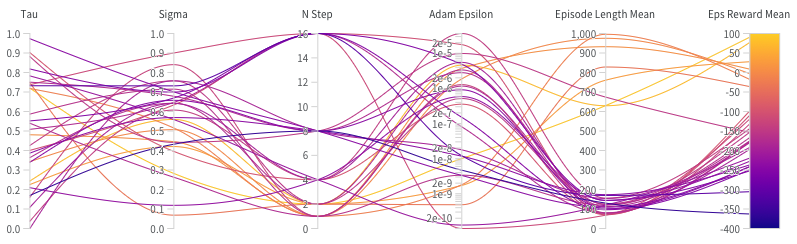
\includegraphics[width=.95\linewidth]{para_coord_baseline_1.png}
		\caption{Lunar Lander Baseline Experiment 1 Hyperparameters}
		\label{fig:baseline_1_para}
	\end{figure}
	Further investigation showed that the observation space assigned to the 
	environment from the RLlib registered lunar lander environment was
	significantly different from the correct space.
	Further, manually registering the environment after importing
	it directly from the Farama maintained packages using Ray's environment
	registration function resulted in an outdated observation space,
	less prone to resulting in error, but still problematic.

	Thus we gain two actionable insights. First, we adjust this experiment 
	to use the custom Lunar Lander environment described in the next section, 
	but set to one agent. Second, we identify an update that can be performed 
	by a pull request to the maintainers of RLlib, a contribution to the 
	open-source software I would like to attempt after the submission of this
	exam.
	
	\subsubsection*{Round 2 - Baseline Parameter Sweep:}
	To evaluate the parameters of the sweep I elect to  conduct a 
	comparison with three different methods. I will use the same methods 
	for the sweeps performed on the subsequent questions as well.
	
	As above, the parallel coordinates graph provides a visual comparison
	of parameter values and a qualitative impression of the effects.
	Second, I use the wandb api Parameter importance and correlation graph,
	which provides an importance metric based on an algorithm from
	\cite{howard2020deep} that combines a tree-based regression and 
	Spearman rank correlation; and the standard	and Pearson correlation
	metric. Finally, for a more quantitative metric I produce an ANOVA 
	table using second order interactions of the hyperparameters.
	
	\begin{figure}
		\centering
		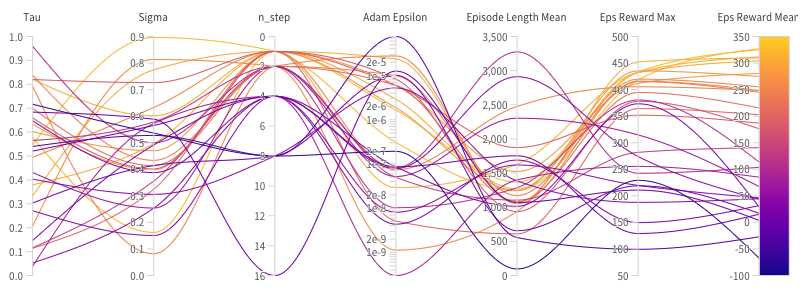
\includegraphics[width=.95\linewidth]{para_coord_baseline_2.png}
		\caption{Lunar Lander Baseline Experiment 2 Hyperparameters}
		\label{fig:baseline_2_para}
	\end{figure}
	\begin{figure}
		\centering
		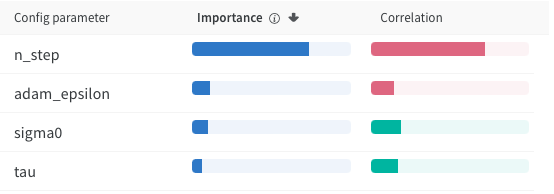
\includegraphics[width=.5\linewidth]{importance_baseline_2.png}
		\caption{Baseline Experiment 2 Hyperparameter Importance}
		\label{fig:baseline_2_importance}
	\end{figure}
	
	\Cref{fig:baseline_2_para} shows the parallel coordinates for this 
	experiment's parameter sweep. Immediately this suggests that 
	the n-step instances under-perform the single step instances.
	The factor importance (\cref{fig:baseline_2_importance}) corroborates this.
	Finally, we execute the ANOVA in \cref{tab:anova_baseline},
	and find that the \(\sigma\) parameter has a statistically significant
	effect on the final performance, particular as an interaction variable.
\end{questions}

\subsection*{Multi-Agent Lunar Lander}
\label{sec:ma-lander}
\addcontentsline{toc}{subsection}{\nameref{sec:ma-lander}}

To modify the Lunar Lander environment to support multiple 
agents it appeared to be possible to simply duplicate all of the
sections that referenced the lander in the original code.
However, to achieve cleaner code, and behavior more consistent with 
Farama's PettingZoo environments, I elected to rewrite the environment
to be more consistent with object oriented programming principles.

\begin{figure}[h]
	\begin{subfigure}{.48\textwidth}
		\centering
		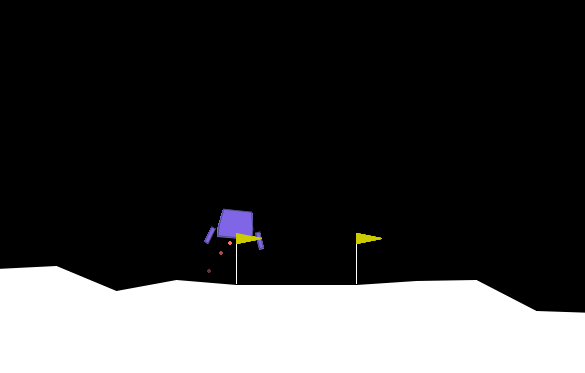
\includegraphics[width=.75\linewidth]{single_lander.png}
		\caption{Original}
		\label{fig:original}
	\end{subfigure}
	\begin{subfigure}{.48\textwidth}
		\centering
		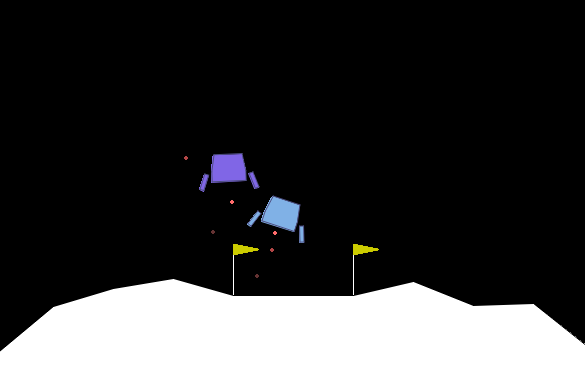
\includegraphics[width=.75\linewidth]{dual_lander.png}
		\caption{With 2 Landers}
	\end{subfigure}
	\\
	\begin{subfigure}{.48\textwidth}
		\centering
		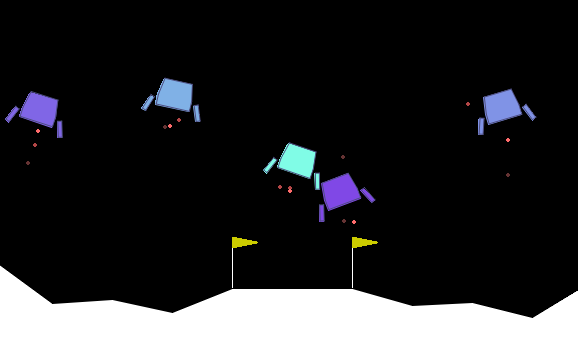
\includegraphics[width=.75\linewidth]{penta_lander_1.png}
		\caption{With 5 Landers}
	\end{subfigure}
	\begin{subfigure}{.48\textwidth}
		\centering
		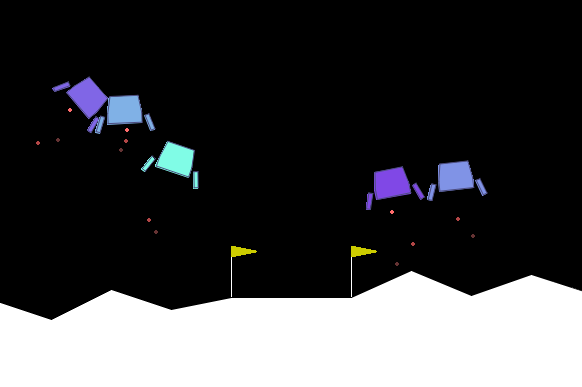
\includegraphics[width=.75\linewidth]{penta_lander_2.png}
		\caption{5 Landers with Collision}
	\end{subfigure}
	\caption{Multi-Agent Lunar Lander}
	\label{fig:landers}
\end{figure}

This trivialized the retention of the environmental physics,
and made it very easy for the new environment to comply with both the 
AEC (Agent Environment Cycle; or sequential) and parallel execution 
methods used in the PettingZoo API. Further, this made it much easier 
to retain the heuristic solution from the original environment.
\Cref{fig:landers} shows several screen shots from the resulting environment
when rendered. 

While an AEC version of this custom environment was constructed,
it was not used for this exam. AEC iterates through the list of agents, 
allowing the agent to select an action and steps the environment with that 
action before moving to the next agent, in a manner similar to a board game.
Such an implement doesn't necessarily contribute value to the 
multi agent Lunar Lander sim, and in fact, causes problems if the physics
of the environment are not adjusted as the number of landers is increased.
Using the heuristic as a measure, the AEC environment becomes unsolvable
with 3 or more landers. The effect of their actions must be scaled to overcome
the wait time between their turns, otherwise they simple crash, unable to 
overcome gravity.

The parallel version of the environment was used for this exam, and required 
only one major assumption, centering around collisions between the landers. 
Lunar Lander uses the Box2D package to model the moon surface and lander.
The most expedient method to address collisions using Box2D was to detect
only contact with the lander's body.
If any other object touches a lander's body it is considered a crash.
As written, the Box2D contact detection does not distinguish between 
what the secondary object is, if the legs of the lander where
included, contact with lunar surface would show as a crash.
Thus I chose not to include the legs contact detection for collisions.
The effective result is that if two lander's legs touch it is not treated
as a crash, however, if one lander's legs touch another's body module
it is treated as a crash and thus a failure.

In addition to being available on the associated github, the new environment
code is included in \cref{app:ma_lander}

\begin{questions}
\setcounter{question}{1}
	\question \textbf{Formulate a Markov Game:}
	The Markov game that represents the multi-agent version of this
	environment is an extension of the Markov Decision Process (MDP)
	that represents the original Lunar Lander environment.
	The formulation presented here will be used to describe the 
	interactions in all of the questions that follow.

	\emph{Agent:} The agent is represented as a member of set of agents 
	\(n\in N\).

	\emph{State Space:} Let \(\mathcal{S}\) be the state space. 
	Then, \(\mathcal{S} \equiv s^N\), where 
	\[s = \begin{cases}
		x \in [-2.5,2.5]   & \text{Position of } n \text{ in } x \\
		y \in [-2.5,2.5]   & \text{Position of } n \text{ in } y \\
		\vec{x} \in [-10,10] & \text{Velocity of } n \text{ in } x \\
		\vec{y} \in [-10,10] & \text{Velocity of } n \text{ in } y \\
		\omega \in [-2\pi,2\pi] & \text{Angle of } n\\
		\vec{\omega} \in [-10,10] & \text{Angular Velocity of } n\\
		\mathbb{I}(\text{leg 1}) \in\{0,1\}  & \text{Leg on ground}\\
		\mathbb{I}(\text{leg 2}) \in\{0,1\}  & \text{Leg on ground}
	\end{cases}\]

	\emph{Action Space:} Let \(\mathcal{A}\) be the action space.
	Then, \(\mathcal{A} \equiv a^N\), where 
	\[a \in \begin{cases}
		0 & \text{No-Op} \\
		1 & \text{Fire Left Engine} \\
		2 & \text{Fire Main Engine} \\
		3 & \text{Fire Right Engine}
	\end{cases}\]

	\emph{Transition Probability:} The transition probability for
	each agent \(n\) remains the same as the original environment,
	\[P_n(s_{n,t+1}|s_{n,t},a_{n,t}) \cong \begin{cases}
		\text{Dispersion} \sim U(-1,1) \\
		\text{Wind(Linear)} = \tanh(\sin(2 k x) + \sin(\pi k x)) \\
		\text{Wind(Rotate)} = \tanh(\sin(2 k x) + \sin(\pi k x)) \\
	\end{cases}\]
	Thus the transition probability for the game as a whole is
	\[P(s_{t+1}|s_{t},a_{t}) = \prod_{n\in N} P_n\]

	\emph{Reward:} The reward structure is similarly retained from 
	the original Lunar Lander environment. Specifically, the reward
	at time \(t\) is defined as
	\(r(t) = \sum_{n\in N} r_n(t)\)
	where
	\begin{align*}
        r_n(t) = \\
        & \pm 100                   & \text{End-state, crash or land} \\
        & +10 (s_{t,6} + s_{t,7})   & \text{leg(s) on ground} \\
        & -a_n(t)\cdot [0,0.03,0.3,0.03] & \text{thruster cost} \\
        & - 100\sqrt{s_{n}(t)_0^2+s_{n}(t)_1^2} & \text{Distance} \\
        & - 100\sqrt{s_{n}(t)_2^2+s_{n}(t)_3^2} & \text{Velocity} \\
        & - 100|\omega_n(t)| & \text{Tilt}
    \end{align*}


    \question \textbf{DQN Single-Agent Controller:}
    This problem was approached using a wrapper class around the
    custom multi-agent environment to translate the between the 
    multi-agent environment and single-agent policy. 
    The proxy single-agent state/observation was formed by simply 
    concatenating the state vectors of each agent.

    The modified action space for this problem is
    \(\mathcal{B} \equiv \mathcal{A}^N\).
    To relate the two action spaces for this problem I use the function,
    \[ b = \sum_{}^{} a_n \times \dim(a)^n. \]
    Then to translate the modified action into the agent-action vector 
    necessary for the multi-agent environment I use the following function,
    \[ \mathbf{a} = \{b/\dim(a)^n \mod\dim(a) \}_{n\in N} \] which 
    relies on \(\dim(\mathcal{A}_n)=\dim(\mathcal{A}_m)\forall\ n,m\in N\),
    an assumption that I note as it is true for this problem, 
    limits some generality.
    The policy can thus be represented as \(\pi(b \big| [s_n]_{n\in N})\).

    Finally, the experiment can be replicated using the command:	
\mint{bash}|python dqn_exp.py --SA --sweep --num-samples=30 --num-env-runners=10|
%
    \begin{figure}
        \centering
        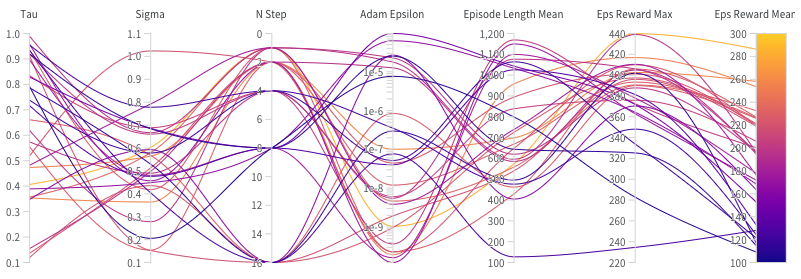
\includegraphics[width=.90\linewidth]{para_coord_sa.png}
        \caption{Single-agent Control Hyperparameter Sweep}
        \label{fig:sa_para}
    \end{figure}
    \begin{figure}
        \centering
        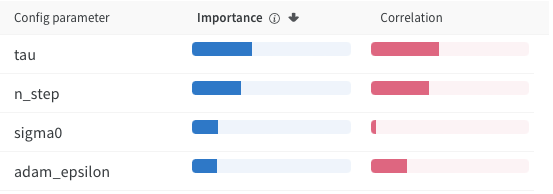
\includegraphics[width=.5\linewidth]{importance_sa.png}
        \caption{Single-agent Control Hyperparameter Importance}
        \label{fig:sa_importance}
    \end{figure}
%
    \Cref{fig:sa_para} shows the results of the parameter sweep for this
    experiment. It appears from this information that there are no clear
    patterns suggesting what the optimal values are for the hyperparameters.
    Next, we consult \cref{fig:sa_importance}. 
    From these metrics we do 
    see some indication that the \(\tau\) and \(n\)-step parameters
    may hold some importance for the final performance.
    And finally, the ANOVA table in \cref{tab:anova_sa}, shows 
    a statistical significance associated with the \(\sigma\)
    parameter. 

    I interpret the high statistical significance but extremely low
    correlation of the \(\sigma\) parameter to suggest that the mid-%
    distribution value has a tendency to produce the best results.
    The superlative instance has a \(\sigma\) parameter near this \(0.5\),
    but overall, it appears that the algorithm is fairly resilient
    to Hyperparameter tuning.


    \question \textbf{NoPS - No Parameter Sharing:}
    This experiment uses a distinct policy for each agent, 
    \(\pi_n(a_n|s_n)\), and can be replicated using:
\mint{bash}|python src/dqn_exp.py --NoPS --sweep --num-samples=30 --num-env-runners=10|
%
    \begin{figure}
        \centering
        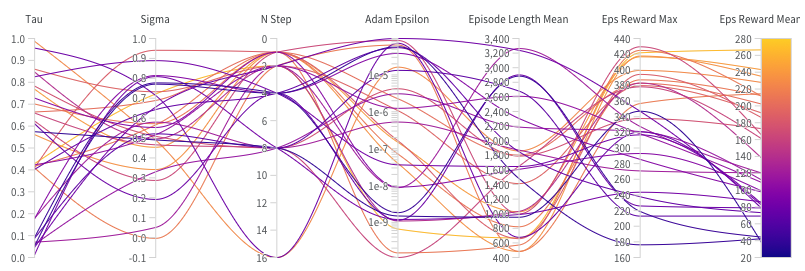
\includegraphics[width=.95\linewidth]{para_coord_nops.png}
        \caption{No Parameter Sharing Hyperparameter Sweep}
        \label{fig:nops_para}
    \end{figure}
%
    The parameter sweep results for this experiment can be seen in 
    \cref{fig:nops_para}. There doesn't appear to be any extremely 
    clear or significant patterns from this parallel comparison.

    There are, however, several observations of interest that are not
    directly concerning the hyperparameters. First, is a generally poor 
    performance for instances that produce longer average episode length.
    Second, unlike the parameter sharing control, this consistently converged
    on a result that produced a positive reward in every case.
    I attribute this partially to sample size, but also note that this
    result is consistent with have two separate policies; that in order
    for the final mean episode reward to be negative, both policies would 
    have to converge to poor behavior.
    This may also explain the more even distribution of average returns
    between the instances of this experiment.

    \begin{figure}
        \centering
        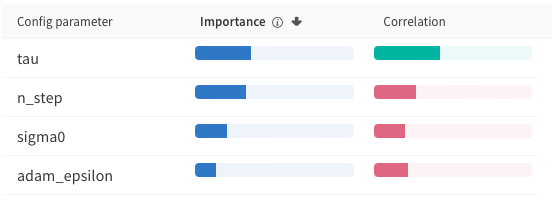
\includegraphics[width=.5\linewidth]{importance_nops.png}
        \caption{No Parameter Sharing Hyperparameter Importance}
        \label{fig:nops_importance}
    \end{figure}

    \begin{figure}%[H]
        \begin{subfigure}{.48\textwidth}
            \centering
            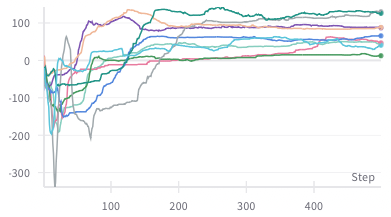
\includegraphics[width=\linewidth]{learn_curve_nops_0.png}
            \caption{Agent 0 Reward}
        \end{subfigure}
        \begin{subfigure}{.48\textwidth}
            \centering
            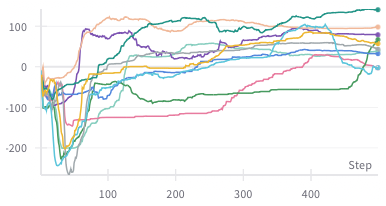
\includegraphics[width=\linewidth]{learn_curve_nops_1.png}
            \caption{Agent 1 Reward}
        \end{subfigure}
        \caption{No-parameter Sharing Learning Curves, 
            average reward \(\times\) training iteration}
        \label{fig:nops_learn_curves}
    \end{figure}

    Next, \cref{fig:nops_importance} shows the parameter importance metrics,
    which similarly suggests no strong relation between the Hyperparameter
    values and results, which is further corroborated in \cref{tab:anova_nops}
    which shows no statistically significant first or second order
    relationship between between the parameters and the final results.
%
    Finally, I present \cref{fig:nops_learn_curves} which shows the learning 
    curves of the agents from 10 instances of this experiment. 
    The resulting curves are consistent with pairs of agents that are
    learning differently. \\ \\ 

    \phantom{text} \\ \\


    \question \textbf{FuPS - Full Parameter Sharing:}
    This experiment uses a shared policy for each agent, 
    \(\pi(a_n|s_n)\), and can be replicated using:
\mint{bash}|python src/dqn_exp.py --FuPS --sweep --num-samples=30 --num-env-runners=10|

    \begin{figure}
        \centering
        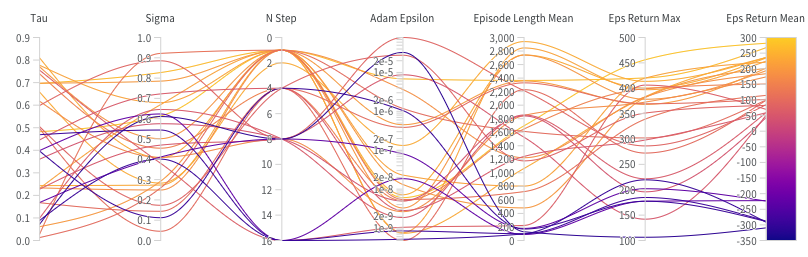
\includegraphics[width=.95\linewidth]{para_coord_fups.png}
        \caption{Full Parameter Sharing Hyperparameter Sweep}
        \label{fig:fups_para}
    \end{figure}

    \begin{figure}
        \centering
        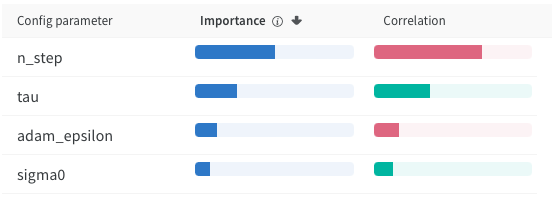
\includegraphics[width=.5\linewidth]{importance_fups.png}
        \caption{Full Parameter Sharing Hyperparameter Importance}
        \label{fig:fups_importance}
    \end{figure}

    The parameter sweep results for this experiment can be seen in 
    \cref{fig:fups_para}, once again it appears that there is a 
    slightly higher performance result from a low or no n-step parameter.
    Further, when considering the additional compute required to execute
    the higher \(n\) instances, it is likely to be net negative.
    \Cref{fig:fups_importance} supports the high performance from lower \(n\).
    Further, between the two figures, some support in favor of a \(\tau>0.5\).
    However, the ANOVA results (\cref{tab:anova_fups}) suggest that these
    may not be statistically significant.

\question \textbf{Results Comparisons:}

    \begin{table}[h]
        \centering
        \begin{tabular}{l cccc}
            Control & \(\tau\) & \(\sigma\) & N-Step & Adam-\(\epsilon\) \\
            \midrule
            Single Agent & 0.5 & 0.6 & 1 & 1e-5\\
            NoPS & 0.75 & 0.5 & 1 & 1e-7 \\
            FuPS & 0.75 & 0.5 & 1 & 1e-8 \\
        \end{tabular}
        \caption{Hyperparameters used for control comparisons.}
        \label{tab:comp_parameters}
    \end{table}

For the comparison I ran 10 instances of each algorithm using the 
parameters in \cref{tab:comp_parameters}, which were values near 
those of the superlative performers in the previous sections.
Some consideration was given to the default values of the DQN implementation. 
It may be noted that Mnih et al. \cite{mnih2015} intended for their algorithm 
to be resilient and require minimal adjustments.
The results seen in the previous sections seem to fit that intent,
with exception to certain more extreme settings.

\begin{figure}[b]
    \centering
    \begin{subfigure}{.48\textwidth}
        \centering
        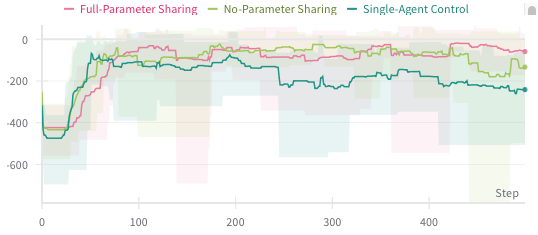
\includegraphics[width=\linewidth]{ep_return_min.png}
        \caption{Minimum Return}
    \end{subfigure}
    \hfil
    \begin{subfigure}{.48\textwidth}
        \centering
        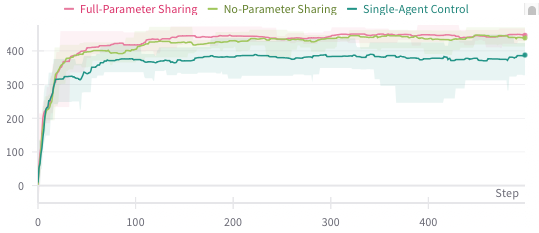
\includegraphics[width=\linewidth]{ep_return_max.png}
        \caption{Maximum Return}
    \end{subfigure}
    \begin{subfigure}{.65\textwidth}
        \centering
        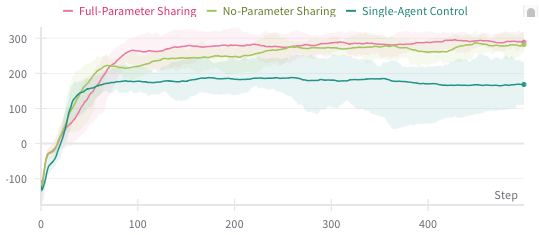
\includegraphics[width=\linewidth]{ep_return_mean.png}
        \caption{Mean Return}
    \end{subfigure}
    \caption{Returns by Episodes}
    \label{fig:ep_returns}
\end{figure}

\Cref{fig:ep_returns} shows learning curve aggregates for each of the 
evaluated algorithms.
From these results we see that the single-agent consistently 
under-performing the other algorithms, particularly, that after 
250 episodes every instance's average was below the average of every 
instance of the other algorithms.
Additionally, the variance in the average performance of the single-agent
control algorithm was significantly greater than the other two algorithms.
I attribute both of these observations to the larger action space and reduced
ability to explore when using this control method.

\begin{figure}
    \centering
    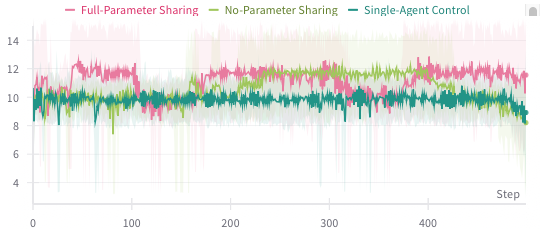
\includegraphics[width=.63\linewidth]{cpu_use.png}
    \caption{CPU Utilization}
    \label{fig:cpu_use}
\end{figure}

\Cref{fig:cpu_use} shows a measure of performance of the algorithms 
from the perspective of computational requirements.
The CPU utilization for the single-agent control was by far the most 
consistent of the three, where the full-parameter sharing was generally
higher while occasionally dropping to a utilization similar to the 
single-agent control. No-parameter sharing appears to have spent equal
time between these two values. 
It is unclear from the experiments conducted for this exam why this would
be the case. I would have expected that the NoPS instance would 
have a generally higher utilization than the others.

\begin{figure}
    \centering
    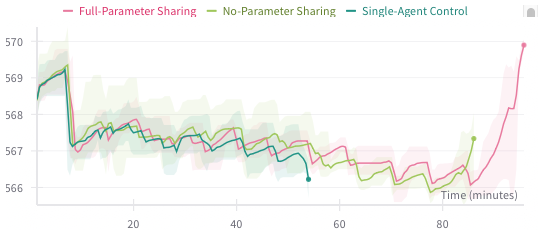
\includegraphics[width=.63\linewidth]{memory_use.png}
    \caption{Memory Usage (MB)}
    \label{fig:memory_use}
\end{figure}

The memory utilization is about the same for each algorithm 
(\cref{fig:memory_use}). Given that the algorithms use the same deep network 
architecture for their value functions, it reasonably follows that the memory 
usage would be similar, with small differences by the nature of the non-sharing 
networks are two separate networks it would not be surprising for those 
instances to have greater memory use, which appears to be the case by a
small margin.

This same graph highlights perhaps the most significant advantage of 
the single agent control, which was an execution time almost half
as long as the others. While this was not an advantage that I had 
considered prior to the experiment it seems that it would follow
that the single agent controller uses the DQN once per step for each 
action and afterwards updates one network, where as the others would 
have to do so twice.

\end{questions}



%%%%%%%%%%%%%%%%%%%%%%%%%%%%%%%%%%%%%%%%%%%%%%%%%%%%%%%%%%%%%%%%%%%%%%%%%%%%%%%%
% --------------------------------- Edit Bar --------------------------------- %
%%%%%%%%%%%%%%%%%%%%%%%%%%%%%%%%%%%%%%%%%%%%%%%%%%%%%%%%%%%%%%%%%%%%%%%%%%%%%%%%











\clearpage
\section{Dr. Cox's Questions}
\begin{questions}
    \question

    I concur with the probable necessity of narrowing the scope of 
    contribution one, particularly to maintain the feasibility of the 
    proposed timeline.

    \begin{parts}
        \part \textbf{Cooperative Tasks:}
            The SISL (Stanford Intelligent Systems Laboratory) environments
            are presented by Gupta et. al. in \cite{gupta2017cooperative}.
            Two of the task in particular I believe to be usable, 
            \emph{Pursuit} and \emph{Waterworld}. The latter of the two 
            can be instantiated as a cooperate-competitive task.
            \emph{Multiwalker} may be included, but that will be determined
            by whether or no I am able to get the task to function as
            expected with different numbers of walkers from the default 3.
            The two former environments are known to operate with a wide
            range of numbers of agents.

            The MPE (Multi Particle Environment) is simple and has a variety
            of available tasks. However, among the manufacturer included
            tasks, \emph{Simple Spread} is probably the only one suitable
            for the proposed evaluated. \emph{Simple Spread} is a 
            task that is essentially a zone-coverage/task-assignment
            type problem.

        \part \textbf{Competitive Tasks:}
            To maintain a greater focus on the adaptability and cooperation
            aspect of agent-groups I believe that it would be best to omit
            any pure competitive tasks. 
            However, I intend to include cooperative-competitive tasks.
            As an example of this, let us take \emph{Water World};
            when the task is set such that a single agent can complete
            (`consume the food') it becomes a pure competitive environment,
            however, increasing that value is intended to produce emergent
            cooperation as the goal requires \(n\) agents to simultaneously
            activate the goal.
        \part \textbf{Algorithms:}
            \begin{table}
                \begin{tabular}{cccc}
                    Base Algorithm & MARL & HARL & Action Space \\
                    PPO & MAPPO & HAPPO & \\
                    DQN & & & 
                \end{tabular}
            \end{table}
        \part \textbf{Environments:}
            
            % Water World - Cont. Action
            % Pursuit - Disc. Action
            % MPE - Disc. Action
            % Smax?
            % MAgent % https://marllib.readthedocs.io/en/latest/handbook/env.html#air-combat
            % Close Air Combat % https://github.com/liuqh16/CloseAirCombat
            % GRF (Research Football)
            % Robot Warehouse? (Jumanji Env.)
        \part \textbf{League:}
            % Agree here that scope may need to narrow, 
            % possible to re-attack as a later paper
    \end{parts}
    \question
\end{questions}

\begin{comment}
Problem 1:


Contribution 1 seems very broadly scoped, and somewhat ill defined (especially when compared
to the well-defined and scoped contribution 2). Please add, at least the following, explicit details
to contribution 1 in terms of:
a. Which cooperative tasks will be explored?
b. Which competitive tasks will be explored?
c. Which algorithms will be explored?
d. Which environments will be explored?
e. Which league frameworks will be explored?
Overall, I am looking for a significant expansion of the methodology of contribution 1 similar to
what we would expect from the final manuscript. Since Contribution 1’s timeline overlaps
significantly with June and July it is reasonable that such details should exist or can be developed.
My concern is that contribution 1 may need to be rescoped to a narrower focus, or split into
multiple papers each with a tighter focus.



Problem 2:


Execute a very small practical experiment of contribution 1: For example, choose 1 MARL
algorithm and 1 HARL algorithm, choose 1 environment with a cooperative task. Write up a minipaper on this experiment. 
You should have an introduction that motivates the problem, a brief
literature review, a detailed methodology section along with a summary of results. 
The goal of this question is to test your ability to implement a very small scale 
experiment aligned with your
proposed contribution 1.




\end{comment}


\clearpage
\addcontentsline{toc}{section}{References}
\printbibliography

\clearpage
\appendix

\section{Experiment Running Script}
\label{app:dqn_exp}
\inputminted[
	fontsize=\footnotesize,
	%bgcolor=gray!05,
	linenos
	]{python3}{../src/dqn_exp.py}

\clearpage
\section{Multi-Agent Lunar Lander}
\label{app:ma_lander}
\inputminted[fontsize=\footnotesize, linenos]{python}{../src/multi_lander.py}

\clearpage
\section{ANOVA Tables}
\label{app:anova_tables}
\scriptsize

\subsection{Baseline Lander}
\label{tab:anova_baseline}
\begin{verbatim}
    OLS Regression Results                            
    ==============================================================================
    Dep. Variable:                  Score   R-squared:                       0.966
    Model:                            OLS   Adj. R-squared:                  0.902
    Method:                 Least Squares   F-statistic:                     15.12
    Date:                Mon, 22 Jul 2024   Prob (F-statistic):           5.46e-05
    Time:                        22:33:51   Log-Likelihood:                -131.47
    No. Observations:                  30   AIC:                             302.9
    Df Residuals:                      10   BIC:                             331.0
    Df Model:                          19                                         
    Covariance Type:            nonrobust                                         
    ========================================================================================
                                coef    std err          t      P>|t|      [0.025      0.975]
    ----------------------------------------------------------------------------------------
    Intercept               70.1409    135.922      0.516      0.617    -232.712     372.994
    tau                  -5.201e+07   2.25e+07     -2.313      0.043   -1.02e+08    -1.9e+06
    sigma                   33.4494     24.068      1.390      0.195     -20.178      87.077
    n_step                 844.5087    373.852      2.259      0.047      11.515    1677.502
    adam_eps               891.1404    278.946      3.195      0.010     269.611    1512.670
    ep_len_mean             -0.0763      0.129     -0.589      0.569      -0.365       0.212
    tau_pow_2             1020.8171    418.234      2.441      0.035      88.934    1952.700
    tau_sigma             2.216e+06   1.12e+06      1.981      0.076   -2.76e+05    4.71e+06
    tau_n_step            1.156e+07    7.5e+06      1.542      0.154   -5.15e+06    2.83e+07
    tau_adam_eps            4.7e+07   2.06e+07      2.283      0.046    1.12e+06    9.29e+07
    tau_ep_len_mean       3824.1099   8513.828      0.449      0.663   -1.51e+04    2.28e+04
    sigma_pow_2              5.0039      1.093      4.580      0.001       2.569       7.438
    sigma_n_step          -158.6486     39.804     -3.986      0.003    -247.337     -69.960
    sigma_adam_eps         -66.9395     34.419     -1.945      0.080    -143.629       9.750
    sigma_ep_len_mean       -0.0181      0.008     -2.187      0.054      -0.037       0.000
    n_step_pow_2           -37.5373    228.941     -0.164      0.873    -547.650     472.576
    n_step_adam_eps      -1089.7884    257.119     -4.238      0.002   -1662.686    -516.891
    n_step_ep_len_mean      -0.0624      0.116     -0.539      0.602      -0.320       0.195
    adam_eps_pow_2        -123.4370    238.454     -0.518      0.616    -654.745     407.871
    adam_eps_ep_len_mean    -0.0525      0.071     -0.740      0.476      -0.211       0.106
    ep_len_mean_pow_2     3.182e-05   2.77e-05      1.150      0.277   -2.98e-05    9.35e-05
    ==============================================================================
    Omnibus:                        5.720   Durbin-Watson:                   1.321
    Prob(Omnibus):                  0.057   Jarque-Bera (JB):                4.528
    Skew:                          -0.944   Prob(JB):                        0.104
    Kurtosis:                       3.246   Cond. No.                     6.21e+16
    ==============================================================================

    Notes:
    [1] Standard Errors assume that the covariance matrix of the errors is correctly specified.
    [2] The smallest eigenvalue is 8.67e-20. This might indicate that there are
    strong multicollinearity problems or that the design matrix is singular.
\end{verbatim}

\clearpage
\subsection{Single-Agent Control}
\label{tab:anova_sa}
\begin{verbatim}
    OLS Regression Results                            
    ==============================================================================
    Dep. Variable:                  Score   R-squared:                       0.868
    Model:                            OLS   Adj. R-squared:                  0.616
    Method:                 Least Squares   F-statistic:                     3.449
    Date:                Tue, 23 Jul 2024   Prob (F-statistic):             0.0247
    Time:                        22:13:46   Log-Likelihood:                -123.07
    No. Observations:                  30   AIC:                             286.1
    Df Residuals:                      10   BIC:                             314.2
    Df Model:                          19                                         
    Covariance Type:            nonrobust                                         
    ========================================================================================
                               coef    std err          t      P>|t|      [0.025      0.975]
    ----------------------------------------------------------------------------------------
    Intercept              415.8797    180.210      2.308      0.044      14.346     817.413
    tau                   1.001e+04   1.98e+06      0.005      0.996   -4.39e+06    4.41e+06
    sigma                  -62.7730     18.266     -3.437      0.006    -103.473     -22.073
    n_step                -168.8124    259.877     -0.650      0.531    -747.856     410.231
    adam_eps                87.5099    200.547      0.436      0.672    -359.336     534.356
    ep_len_mean              0.1006      0.244      0.413      0.688      -0.442       0.643
    tau_pow_2              311.4753    314.546      0.990      0.345    -389.377    1012.328
    tau_sigma            -2.468e+04   2.05e+05     -0.121      0.906   -4.81e+05    4.31e+05
    tau_n_step            9.437e+06   6.03e+06      1.566      0.148   -3.99e+06    2.29e+07
    tau_adam_eps         -4.769e+06   3.13e+06     -1.522      0.159   -1.18e+07    2.21e+06
    tau_ep_len_mean      -2349.7876   2023.141     -1.161      0.272   -6857.627    2158.052
    sigma_pow_2              2.4038      0.599      4.012      0.002       1.069       3.739
    sigma_n_step             1.2135     10.117      0.120      0.907     -21.329      23.756
    sigma_adam_eps           8.5121      5.914      1.439      0.181      -4.665      21.689
    sigma_ep_len_mean        0.0263      0.010      2.674      0.023       0.004       0.048
    n_step_pow_2            53.2984    129.963      0.410      0.690    -236.278     342.875
    n_step_adam_eps        231.7169    252.934      0.916      0.381    -331.855     795.289
    n_step_ep_len_mean      -0.0407      0.226     -0.180      0.861      -0.545       0.464
    adam_eps_pow_2        -126.2286    110.253     -1.145      0.279    -371.888     119.430
    adam_eps_ep_len_mean    -0.1330      0.112     -1.188      0.262      -0.383       0.116
    ep_len_mean_pow_2     -8.01e-06      0.000     -0.056      0.957      -0.000       0.000
    ==============================================================================
    Omnibus:                        8.754   Durbin-Watson:                   1.550
    Prob(Omnibus):                  0.013   Jarque-Bera (JB):                7.490
    Skew:                          -0.903   Prob(JB):                       0.0236
    Kurtosis:                       4.651   Cond. No.                     5.78e+15
    ==============================================================================
    
    Notes:
    [1] Standard Errors assume that the covariance matrix of the errors is correctly specified.
    [2] The smallest eigenvalue is 4.72e-19. This might indicate that there are
    strong multicollinearity problems or that the design matrix is singular.
\end{verbatim}

\clearpage
\subsection{No Parameter Sharing}
\label{tab:anova_nops}
\begin{verbatim}
    OLS Regression Results                            
    ==============================================================================
    Dep. Variable:                  Score   R-squared:                       0.864
    Model:                            OLS   Adj. R-squared:                  0.605
    Method:                 Least Squares   F-statistic:                     3.339
    Date:                Tue, 23 Jul 2024   Prob (F-statistic):             0.0276
    Time:                        12:14:05   Log-Likelihood:                -138.94
    No. Observations:                  30   AIC:                             317.9
    Df Residuals:                      10   BIC:                             345.9
    Df Model:                          19                                         
    Covariance Type:            nonrobust                                         
    ========================================================================================
                               coef    std err          t      P>|t|      [0.025      0.975]
    ----------------------------------------------------------------------------------------
    Intercept              425.0804    244.891      1.736      0.113    -120.571     970.732
    tau                  -2.892e+06   2.95e+06     -0.980      0.350   -9.47e+06    3.68e+06
    sigma                  -13.7033     25.615     -0.535      0.604     -70.776      43.370
    n_step                 -60.6324    363.894     -0.167      0.871    -871.440     750.175
    adam_eps              -101.7131    477.938     -0.213      0.836   -1166.626     963.200
    ep_len_mean              0.0414      0.187      0.222      0.829      -0.375       0.458
    tau_pow_2              -73.8498    253.375     -0.291      0.777    -638.404     490.704
    tau_sigma             -9.58e+04   2.43e+05     -0.394      0.702   -6.37e+05    4.45e+05
    tau_n_step           -1.973e+06   4.24e+06     -0.465      0.652   -1.14e+07    7.47e+06
    tau_adam_eps          3.361e+06   3.01e+06      1.117      0.290   -3.34e+06    1.01e+07
    tau_ep_len_mean       1460.5816    946.981      1.542      0.154    -649.424    3570.587
    sigma_pow_2              0.4027      1.422      0.283      0.783      -2.765       3.571
    sigma_n_step           -17.9749     30.768     -0.584      0.572     -86.530      50.580
    sigma_adam_eps          20.5071     19.299      1.063      0.313     -22.494      63.508
    sigma_ep_len_mean        0.0005      0.006      0.087      0.933      -0.012       0.013
    n_step_pow_2             5.5271    268.271      0.021      0.984    -592.218     603.273
    n_step_adam_eps        100.0307    249.637      0.401      0.697    -456.195     656.256
    n_step_ep_len_mean      -0.0024      0.080     -0.030      0.977      -0.180       0.175
    adam_eps_pow_2          46.3900    267.727      0.173      0.866    -550.143     642.923
    adam_eps_ep_len_mean    -0.0622      0.095     -0.654      0.528      -0.274       0.150
    ep_len_mean_pow_2    -2.231e-05   3.99e-05     -0.560      0.588      -0.000    6.65e-05
    ==============================================================================
    Omnibus:                        2.859   Durbin-Watson:                   1.983
    Prob(Omnibus):                  0.239   Jarque-Bera (JB):                1.678
    Skew:                          -0.548   Prob(JB):                        0.432
    Kurtosis:                       3.378   Cond. No.                     1.63e+16
    ==============================================================================
    
    Notes:
    [1] Standard Errors assume that the covariance matrix of the errors is correctly specified.
    [2] The smallest eigenvalue is 2.28e-18. This might indicate that there are
    strong multicollinearity problems or that the design matrix is singular.
\end{verbatim}

\clearpage
\subsection{Full Parameter Sharing}
\label{tab:anova_fups}
\begin{verbatim}
    OLS Regression Results                            
    ==============================================================================
    Dep. Variable:                  Score   R-squared:                       0.953
    Model:                            OLS   Adj. R-squared:                  0.840
    Method:                 Least Squares   F-statistic:                     8.450
    Date:                Tue, 23 Jul 2024   Prob (F-statistic):            0.00219
    Time:                        12:16:56   Log-Likelihood:                -128.54
    No. Observations:                  28   AIC:                             297.1
    Df Residuals:                       8   BIC:                             323.7
    Df Model:                          19                                         
    Covariance Type:            nonrobust                                         
    ========================================================================================
                                coef    std err          t      P>|t|      [0.025      0.975]
    ----------------------------------------------------------------------------------------
    Intercept              175.2457    162.159      1.081      0.311    -198.692     549.184
    tau                    186.4124    296.485      0.629      0.547    -497.284     870.109
    sigma                 1043.0267    402.067      2.594      0.032     115.859    1970.194
    n_step                2.574e+06   9.38e+06      0.274      0.791   -1.91e+07    2.42e+07
    adam_eps               -95.1023     52.882     -1.798      0.110    -217.048      26.843
    ep_len_mean             -0.0065      0.113     -0.057      0.956      -0.266       0.253
    tau_pow_2              190.7520    308.769      0.618      0.554    -521.270     902.774
    tau_sigma              287.9223    339.789      0.847      0.421    -495.633    1071.478
    tau_n_step            2.957e+07   2.43e+07      1.215      0.259   -2.65e+07    8.57e+07
    tau_adam_eps           -11.6668     25.878     -0.451      0.664     -71.341      48.008
    tau_ep_len_mean         -0.1573      0.138     -1.140      0.287      -0.476       0.161
    sigma_pow_2           -723.8557    329.556     -2.196      0.059   -1483.814      36.103
    sigma_n_step          1.668e+07   1.05e+07      1.592      0.150   -7.48e+06    4.08e+07
    sigma_adam_eps         -64.5262     24.704     -2.612      0.031    -121.494      -7.559
    sigma_ep_len_mean       -0.1967      0.106     -1.850      0.101      -0.442       0.048
    n_step_pow_2          6058.0985   5450.747      1.111      0.299   -6511.346    1.86e+04
    n_step_adam_eps      -1.209e+06    1.3e+06     -0.933      0.378    -4.2e+06    1.78e+06
    n_step_ep_len_mean   -1.043e+04   6264.673     -1.665      0.135   -2.49e+04    4018.744
    adam_eps_pow_2           5.8045      2.667      2.176      0.061      -0.346      11.955
    adam_eps_ep_len_mean     0.0344      0.019      1.799      0.110      -0.010       0.078
    ep_len_mean_pow_2     1.923e-05   3.59e-05      0.535      0.607   -6.36e-05       0.000
    ==============================================================================
    Omnibus:                        1.813   Durbin-Watson:                   2.036
    Prob(Omnibus):                  0.404   Jarque-Bera (JB):                1.473
    Skew:                          -0.545   Prob(JB):                        0.479
    Kurtosis:                       2.725   Cond. No.                     1.20e+17
    ==============================================================================

    Notes:
    [1] Standard Errors assume that the covariance matrix of the errors is correctly specified.
    [2] The smallest eigenvalue is 3.25e-20. This might indicate that there are
    strong multicollinearity problems or that the design matrix is singular.
\end{verbatim}

\end{document}
